\documentclass[10pt]{article}
\usepackage[margin=0.65in]{geometry}
\usepackage{graphicx,hyperref,xurl,parskip,amssymb,booktabs}
\hypersetup{colorlinks=true,urlcolor=blue}
\begin{document}
\sloppy
\emergencystretch=3em
\begin{center}\Large Bounded GPU continuation: actual run 0 and run 1\\
\normalsize Audit items 7 and 13; recorded 18 October 2026\end{center}
\textbf{GPU control executed; continuation stopped; original closure censored.}
Run 1 built CUDA13.3.73 and passed native/device checks on RTX5090. Its
original ingestion gate then refused valid zero-length trails. Health,
restart equality, throughput benchmarks and challenge collection did not run.
The original high-memory CPU closure failed allocation without measuring D.

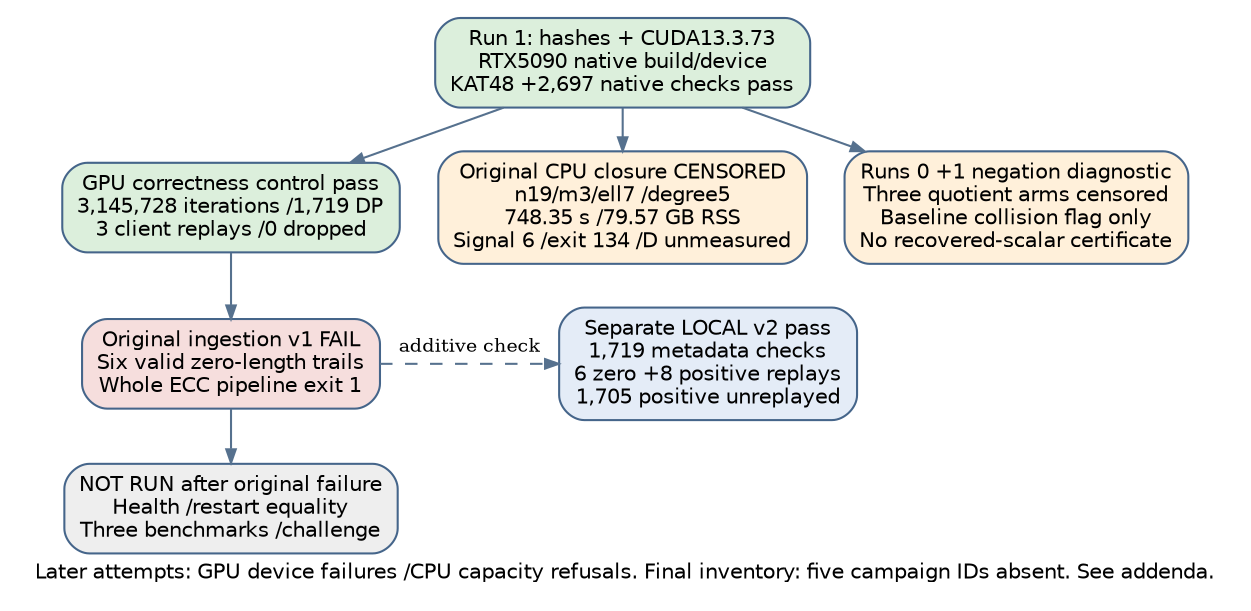
\includegraphics[width=\linewidth]{run-flow.png}

\textbf{Recovered evidence.} Run 0 archive: 15,160 bytes, SHA256 prefix
\texttt{26d26efe1f6e8d99}. Run 1: 139,739 bytes, SHA256 prefix
\texttt{c7ddcdbd1a88c72e}. All 147 run1 manifest files passed independent
hash verification in both retained and freshly extracted trees. Full hashes,
raw commands, resources, failures and source references are in
\texttt{RUN0\_RESULTS.md}, \texttt{RUN1\_RESULTS.md} and
\path{diagnostics/run1-audit/receipt.json}. The controller records deletion
and verified absence of the dedicated pod. No later allocation is represented
as a scientific run here.

\textbf{Identity and runtime.} ECC source is pinned to
\texttt{0ea8931d21d567f83de47c30bdaac0585f479c11} (39 files), public P/Q on
$y^2+xy=x^3+1$ over $\mathbb F_{2^{131}}$, exact native permuted type-II
normal basis and subgroup order 680564733841876926932320129493409985129.
The polynomial-basis registry alias is not substituted. Delivery source:
\texttt{9bb0c292b3b1d6b0fafe9c33f73a2145d3dc4830}. Observed driver 580.65.06,
driver API 13000, runtime 13030. Native doctor/build passes support this actual
configuration, not universal driver compatibility.

\newpage
\begin{center}\large GPU correctness and additive local ingestion\end{center}
Remote host bundle: 2,862 sigma checks including 48/48 public known answers;
28,641 native-CLMUL and28,638 portable controls. Separate native sigma checker:
2,697 checks and 48/48 KAT. The GPU control used run 53180, DP weight 46,
256 threads,16 slots,96 steps and 8 launches. It reported 3,145,728 iterations,
1,719 reports,3 native golden-model replays,0 bad reports and 0 dropped.
The raw 0.213-second interval is a short correctness diagnostic, not a
repeated campaign benchmark or replacement for historical production rates.

The original independent ingester exited 1 with ``invalid trail length.''
Six retained reports have zero length because their seed start is already
DP46. The original remote pipeline remains failed. A separately frozen local
v2 qualification preserves v1 and the run's bytes, checks all 1,719 paired
reports for public-curve/weight/namespace/encoding, and independently replays
\emph{all} 6 zeros plus 8 eligible positive trails. Exactly 1,705 positive trails
remain unreplayed. Seed-tampered zero and coordinate-tampered positive
controls fail. This local correction does not execute any missing remote gate.

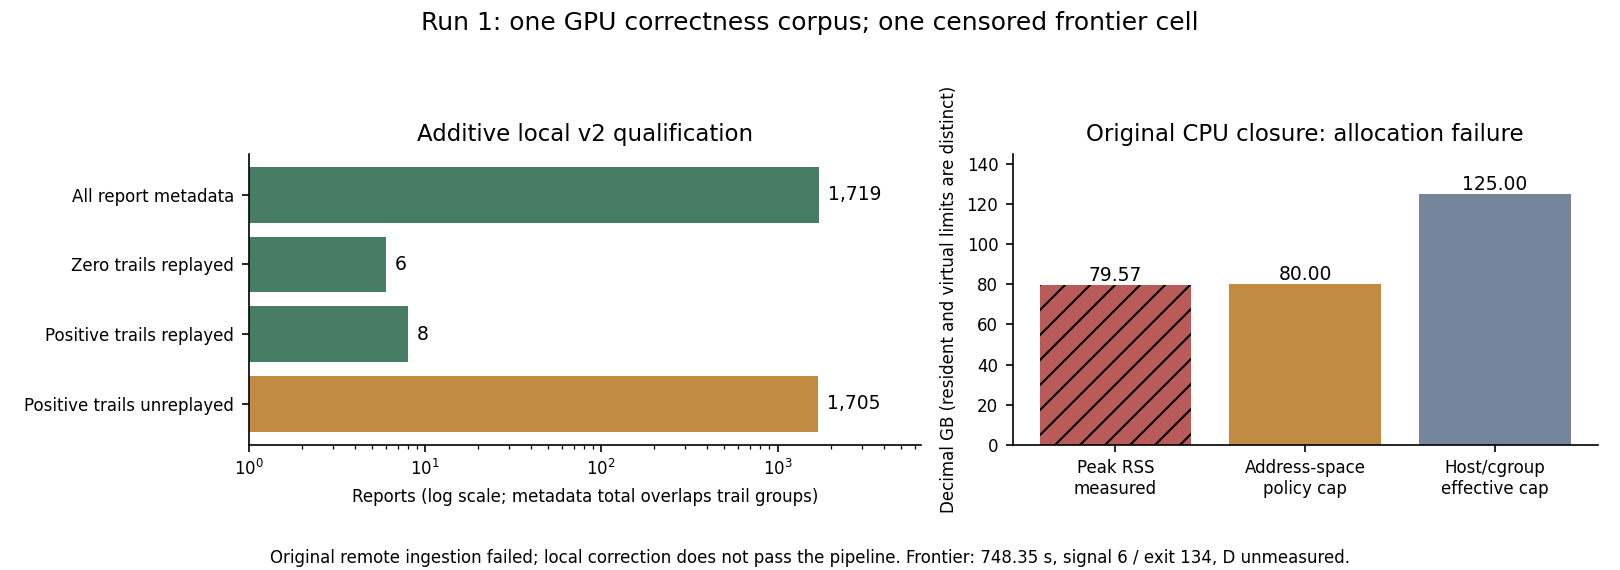
\includegraphics[width=\linewidth]{run1-validation-memory.png}

\textbf{Original memory-frontier attempt.} Committed n19/m3/ell7,draw0,
40 Boolean variables,degree 5,max-columns 800000; native XL/MutantXL closure.
Tiny controls passed: SAT retains 12 solutions through 4, UNSAT refutes at 4.
Effective host limit 124,999,999,488bytes passed the96GB gate. The process
address-space cap was 80,000,000,000bytes. After 748.35 s wall, 700.06 s user
and 49.23 s system CPU, allocation of 3320 bytes failed. Peak RSS 77,709,264 KiB
is 79,574,286,336 bytes. No frontier JSON result was emitted; D remains
\textbf{unmeasured}. No bound on D follows from the failed incomplete scan.

The time log simultaneously says ``Command terminated by signal 6'' and
\texttt{exit\_status:0} from its \texttt{\%x} field. The separate process exit
and terminal receipts say 134. The bare exit-field 0 does not encode signal
termination and is not success; signal 6/actual exit 134 governs the failure.
Both original fields remain retained. This was CPU closure on a GPU host,
not GPU/distributed F4 or an F4 solving-degree measurement; there was no
inner closure checkpoint.

\newpage
\begin{center}\large Run 0 failure, negation diagnostics and remaining criteria\end{center}
Run 0 preserved a packaging failure: omitted protocol/binding documents and
nonexecutable frontier script. All 39 ECC source hashes passed, then hardware
manifest gate exited 1; ECC and frontier were skipped. Four native negation
commands executed. The source packet was corrected additively for run1;
run0's failures remain charged and immutable.

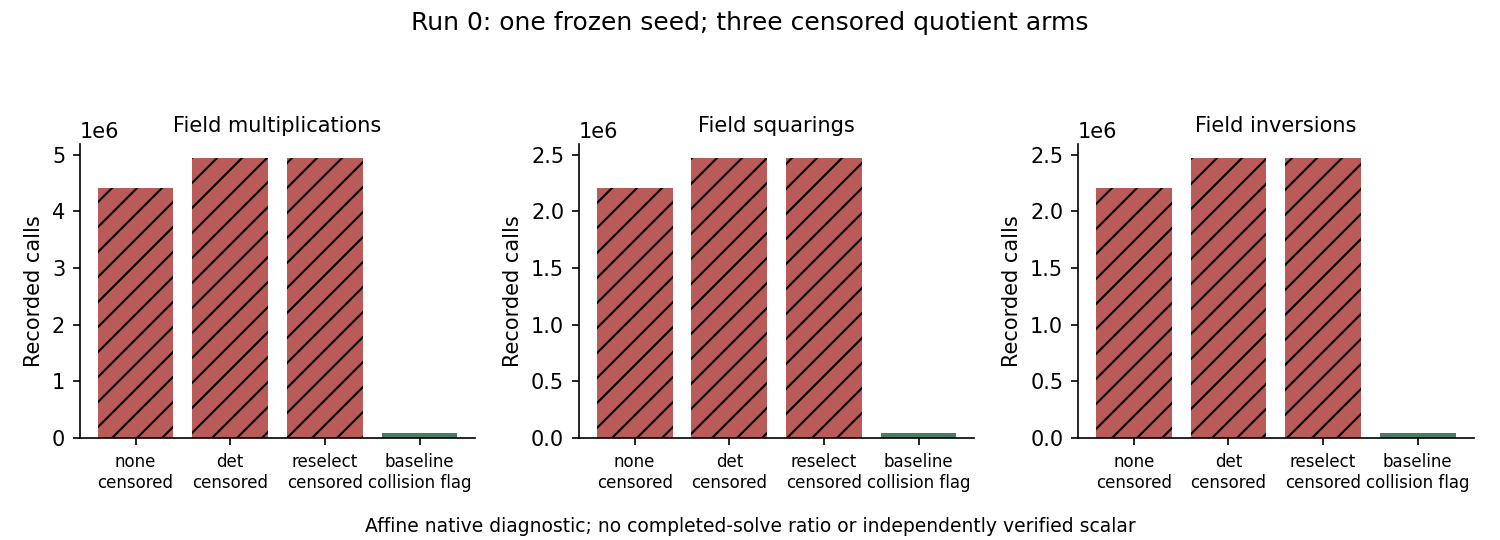
\includegraphics[width=\linewidth]{run0-operation-counters.png}

Run 1 repeats the same diagnostic step/operation/DP/censoring/collision counters
(only deterministic-break peak RSS differs). All three quotient arms hit the
2,208,379-step budget and remain censored. Baseline reports 42,678 steps and
a collision flag without an independently replayed recovered scalar.
A successful command exit is not a completed mathematical solve. The original
H-RHO-bc6ea6/EXP-RHO-60da4f already has substantial prior trials and retains
its affine/Jacobian deviation; this four-arm diagnostic does not close the
full experiment. No completed-solve ratio or M-equivalent gain is inferred.

\textbf{Remaining gates.} A prospectively admitted whole-pipeline rerun with
the corrected checker must pass health, exact checkpoint-restart equality,
three bounded benchmarks, challenge slices and independent ingestion.
Run 53181 remains quarantined, without a global seed lease or shared-store
upload. Long trails require explicit replay scope; collision detection is
not scalar recovery. Finishing ECC2K-130 requires an independently verified
challenge scalar. The original frontier still needs completion with a valid
resource boundary; a smaller substitute cannot discharge that obligation.
Distributed/out-of-core/GPU F4 and the complete negation contract remain open.

\textbf{Graph and claim boundary.} Updated graph sources/renderings are
\path{reports/run-flow.dot} and \path{reports/plot_run1.py}; native-derived
counts are retained in \path{reports/run1-summary.json}. Canonical sources
\path{papers/ecdlp-constant/sec-ecc2k-campaign.tex} and
\path{sec-ecc2k-gpu.tex} were checked. Their historical production rates,
IC leaderboard and forecasts remain current: a short DP46 control and failed
closure are not replacement production measurements. No attack-cost,
asymptotic, speedup, full challenge or scientific state transition is claimed.

\newpage
\begin{center}\large Addendum: split GPU-v3 failed-host attempt\end{center}
\textbf{Separate attempt, 05:41:00--05:41:52 UTC.} Source delivery
\texttt{3e36dca3b10a69f013e97c965f4cec7ed1c1f523}; no original evidence or
run1 finding is rewritten. Archive 27,213 bytes, SHA256 prefix
\texttt{15516ac73ae3b4e7}. All 120 manifest-listed payload files match in
retained and fresh extraction trees; 121 archived files include the manifest.
Full hash and independent checks: \path{diagnostics/gpu-v3-audit/receipt.json}.

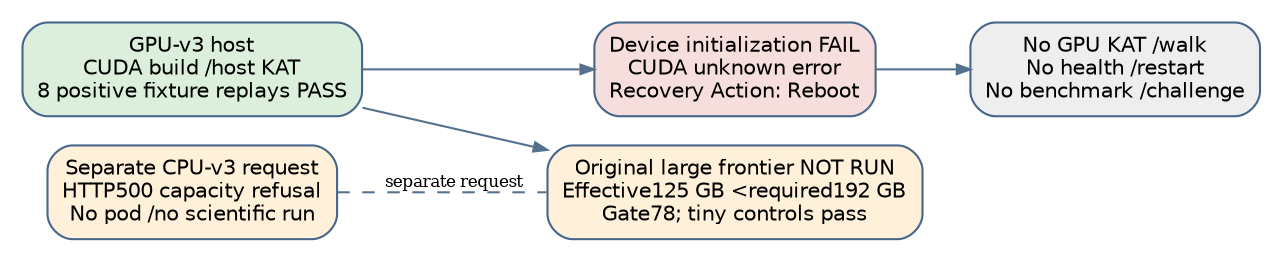
\includegraphics[width=\linewidth]{gpu-v3-flow.png}

\textbf{Build passes, device fails.} CUDA13.3.73 build and host bundle
exited 0: 2,862 sigma checks including48/48 known answers, 28,642 CLMUL and
28,642 portable controls. The remote native v2 positive fixture passed 8 records
and 8 golden replays; it contains no zero-length report. The CUDA device doctor
then exited 3: unknown error, driver API 13000/runtime 13030, devices empty.
Native GPU KAT/checker, GPU walk and GPU-report ingestion did not run.
Health/restart, benchmarks and challenge likewise did not run.

The host's \texttt{nvidia-smi} records RTX5090, driver 580.173.02 and
\textbf{GPU Recovery Action: Reboot}. These observations identify this
failed device-initialization attempt and recovery flag; they do not establish
a general toolchain incompatibility or change run1's earlier successful control.
All four negation commands returned 0; the three quotient arms remain
censored and baseline is a collision flag, not an independently recovered scalar.

\textbf{Memory gate prevents a new large closure.} Physical RAM was
405,163,536,384bytes, but cgroup/effective RAM was 124,999,999,488bytes,
below the revised 192,000,000,000-byte gate. Gate exit 78 records the original
large n19/m3/ell7 cell as unexecuted; tiny SAT/UNSAT controls passed before
that gate. No new frontier measurement or D is supplied. Run1's earlier
allocation failure remains the only large-frontier attempt in this packet.

\textbf{CPU-v3 capacity refused.} The separate 256 GB CPU request received
an actual provider HTTP500 capacity refusal, pod id null. No CPU allocation
or scientific trial occurred. This is an infrastructure refusal, not evidence
about the mathematics. The GPU controller fetched evidence, deleted its pod
and verified absence; an independent watchdog also found absence. Reporting
performed no provider or Git mutation.

\textbf{Current record.} See \texttt{GPU\_V3\_RESULTS.md} and
\path{reports/continuation-summary.json}. The pre-addendum three-page PDF
is preserved as \path{reports/run1-report.pdf}. Original ingestion failure,
separate local v2 qualification and unreplayed-trail limits remain unchanged.
Historical campaign rate figures and forecasts remain unchanged; no throughput,
challenge completion, solving degree, attack gain or scientific transition
is inferred from this failed-host attempt.

\end{document}
